\documentclass[11pt]{article}
\usepackage[margin=2.5cm]{geometry}
\usepackage{booktabs}
\usepackage{amsmath}
\usepackage{hyperref}
\usepackage{graphicx}
\graphicspath{{figures/}}
\usepackage{url}
\setlength{\parskip}{4pt}

\title{Nobody Beats Tuned Uniform: A Mechanism-Level Autopsy\\of Per-Query Retrieval Routing}
\author{ChefSanto\\
  \small AI Lab --- \url{https://github.com/ChefSanto/rags}}
\date{October 2026}

\begin{document}
\maketitle

\begin{abstract}
Per-query retrieval routing --- choosing BM25, dense retrieval, or fusion \emph{per query} --- is motivated by oracle analyses showing large headroom: a cheat that always picks the best strategy per query outperforms the best fixed strategy by 14--17\% relative nDCG on BEIR datasets (honest train/test protocol; 12--13\% under the all-splits convention). We set out to harvest that headroom and failed seven times, each failure in a different way. Across gradient-boosted routers on lexical and embedding features, cross-domain transfer, two generations of pseudo-labeled training data (document sentences and LLM-generated questions), soft routing by per-query fusion-weight regression, and zero-shot LLM routing, \textbf{no router beats a single tuned fusion weight} --- and the best-intentioned variants are \emph{worse} than doing nothing. We diagnose why, mechanism by mechanism: an alphabetical tie-breaking artifact that collapses classifiers; regression that predicts strategy \emph{levels} but never per-query \emph{deviations}; pseudo-queries that are lexical copies of their source documents; a non-convex quality surface in fusion weight that traps weight-regression; and LLM routers that either hedge to the safe answer (fusion) or commit to priors that are anti-predictive on BEIR. A break-even analysis closes the loop: the oracle's wins are abundant (half of all queries) but carry no query-side fingerprint beyond chance, so \emph{any} router built on reading the query operates exactly at its profitability threshold. We validate the stakes at the answer level: retrieval strategy choice propagates to grounded-answer quality, confirmed by a blind 90-judgment human evaluation. The practical recommendation is unfashionable and robust: sweep the weight, ship the constant. The artifact is a complete, deployed RAG platform with which every claim in this paper can be reproduced from a YAML config.
\end{abstract}

\section{Introduction}
Retrieval-Augmented Generation systems are only as good as their retriever, and retrievers disagree. Lexical methods (BM25) excel on terminology-dense queries; dense bi-encoders excel on paraphrased, conceptual questions; hybrid fusion often dominates both. It is natural to ask: \emph{can a router choose the best strategy per query?}

The field's motivating evidence is the \textbf{oracle analysis}: score every strategy on every query, let a cheat pick the per-query maximum, and measure the gap over the best fixed strategy. Gaps of 10--20\% are common, and they have launched a research program of learned routers.

This paper is the controlled study of that program's premise. We built a reproducible experimentation platform (Section~2), established the oracle gap on two BEIR domains (Section~3), and then attempted to capture it with seven router families spanning the design space: feature-based classification and score regression, per-corpus pseudo-labeled training data of two generations, cross-domain transfer, soft routing via per-query fusion weights, and zero-shot LLM routing (Section~4). \textbf{None beats a tuned uniform fusion weight.} Each failure carries a diagnosed mechanism, and the mechanisms --- not just the outcomes --- are the paper's contribution.

Concurrent and independent work (RCT-MARS, published August 2026 while this study was underway) identified the same core paradox --- ``no learned hard router beats the strongest fixed method despite a large oracle ceiling'' --- on a five-strategy, six-benchmark stack, and showed that \emph{soft} routing (learned per-query fusion weights) recovers part of the gap. Our study was conducted independently on a different stack and protocol, reaches the stronger conclusion that \textbf{soft routing fails on BEIR-style train/test splits too} (its most direct variant catastrophically, via a mechanism we document), and adds what a paradox paper cannot: a break-even theory explaining \emph{why} every paradigm lands at zero (Section~5), a human-validated answer-level analysis (Section~6), and an end-to-end artifact.

Our findings in one sentence: \textbf{the oracle gap is real, abundant, and unreachable from query-side information} --- routing's headroom is a measurement of how much knowing the answer would help, not of how much a router can gain.

\subsection{Claims}
\begin{enumerate}
\item On FiQA and NFCorpus, the per-query oracle beats the best fixed strategy by +14--17\% relative nDCG (Section~3, test-split protocol; +12--13\% all-splits); domain labels capture only +1.3\% of it (Section~4.1).
\item Seven router families --- spanning feature, label-generation, soft-weight, and LLM paradigms --- all fail to beat a tuned uniform weight; five are worse than it (Section~4). Two failure mechanisms are, to our knowledge, undocumented: alphabetical tie-breaking bias in argmax labels under dense annotations (\S\ref{sec:v0}), and the non-convex weight-valley that collapses fusion-weight regression (\S\ref{sec:v5}).
\item A break-even analysis explains the flat results: the oracle wins on roughly half of queries; the required pick accuracy is 45--50\%, and trained predictors land at 44--58\% per domain --- at or marginally above break-even (paired bootstrap $P{=}0.95$ pooled), which caps routed gains at ${\approx}{+}0.003$ nDCG (Section~5, reviewer statistics in the artifact).
\item Strategy choice matters at the answer level --- grounding scores and blind human judgments both order dense $>$ hybrid $>$ bm25 identically --- so the routing question is worth asking even though current routers fail it (Section~6).
\item Everything is reproducible from the public artifact (Section~2, Appendix~A).
\end{enumerate}

\section{Setup: platform, data, protocol}
\subsection{The platform}
All experiments run on \textbf{AI Lab}, a deliberately small reproducibility platform (the repository is the artifact). An experiment is a YAML file (dataset, retrieval strategy and parameters, seed, metrics); a runner executes it and writes (a)~a result JSON with metrics and full provenance (git commit, seed, package versions, hardware), and (b)~the ranked run as a machine-readable artifact. Canonical runs execute on Kaggle GPU; results and run artifacts are committed to git, making every analysis in this paper executable from a fresh clone. Retrieval implementations include an inverted-index BM25 with document-frequency filtering, dense retrieval over \texttt{all-MiniLM-L6-v2}, and min--max normalized score fusion.

\subsection{Data and evaluation}
BEIR-format datasets: \textbf{FiQA} (finance, 57{,}638 documents, 6{,}648 queries with judgments) and \textbf{NFCorpus} (biomedical, 3{,}633 documents, 3{,}237 queries). Two complementary evaluation conventions are used and clearly separated:
\begin{itemize}
\item \textbf{All-splits} (train+dev+test merged): for baseline tables and comparability with published BEIR numbers.
\item \textbf{Honest train/test protocol}: qrels are split by BEIR's train/dev/test partition; routers train on \texttt{train} and are evaluated once on \texttt{test}. All router results in this paper use this protocol unless stated.
\end{itemize}
Primary metric: nDCG@10 (judged queries, rel~$\geq$~1 threshold, graded gains), macro-averaged. Oracle analyses use per-query variants of the same functions; sanity checks confirm per-query macro means reproduce the stored metrics exactly.

\subsection{Strategies}
BM25 ($k_1{=}1.5$, $b{=}0.75$), dense (\texttt{all-MiniLM-L6-v2}), and hybrid (min--max fusion, \texttt{dense\_weight} swept in \S\ref{sec:matrix}). The hybrid weight sweep --- a foreshadowing of this paper's conclusion --- found \texttt{dense\_weight}${=}0.7$ optimal on FiQA (nDCG@10 0.3827, beating dense 0.3680 and bm25 0.2293) and 0.5 optimal on NFCorpus (0.3414 vs 0.3186/0.3185).


\section{The oracle gap is real}
Table~\ref{tab:baselines} establishes the phenomenon that motivates routing. On both domains, a per-query oracle --- picking each query's best strategy from the three --- substantially outperforms every fixed strategy.

\begin{table}[h]
\centering\small
\begin{tabular}{lccccc}
\toprule
domain & bm25 & dense & hybrid & best fixed & oracle \\
\midrule
FiQA     & 0.2293 & 0.3680 & 0.3827 @ $w{=}0.7$ & \textbf{0.3827} & 0.4271 \\
NFCorpus & 0.3013 & 0.3183 & 0.3374 @ $w{=}0.5$ & \textbf{0.3374} & 0.3818 \\
\bottomrule
\end{tabular}
\caption{Baselines and oracle under the \emph{all-splits} protocol (train+dev+test merged; comparability with published BEIR numbers). Oracle gaps: +11.6\% relative (FiQA), +13.2\% (NFCorpus). All router results in this paper (Table~\ref{tab:matrix}) use the honest \emph{test-split} protocol instead (gaps +16.9\%/+14.1\%); the phenomenon holds under both.}
\label{tab:baselines}
\end{table}

Head-to-head, no strategy dominates: BM25 beats dense on 31.3\% of NFCorpus queries but only 14.5\% of FiQA queries. The winner \emph{varies} --- the precondition for routing to matter.

Under the honest test-split protocol the pattern holds: oracle 0.4338 (FiQA) and 0.3842 (NFCorpus) vs best-uniform 0.3711 and 0.3368 --- \textbf{+16.9\% and +14.1\% relative} (weighted oracle 0.4173 vs 0.3597). Protocol note: Table~\ref{tab:baselines} is all-splits; Table~\ref{tab:matrix} is test-split; the gap holds under both (\S2.2).

One observation frames everything that follows: the \textbf{soft oracle exceeds the hard oracle}. Allowing per-query fusion weights $w \in \{0, 0.1, \dots, 1.0\}$ (RRF-fused BM25+dense rankings, weight grid-searched per query) reaches 0.4413/0.3884 --- \emph{above} per-query strategy selection (0.4338/0.3842). Fusion hedges: blending two thin, complementary rankings rescues queries no single strategy serves. Quantified per query (reviewer statistics, artifact): the soft oracle beats strategy selection on only 9.6\% (FiQA) and 14.2\% (NFCorpus) of test queries, and the tuned \emph{constant} weight already captures 50.6\% of the positive hedging mass. The oracle is, mostly, a constant fusion with small wiggles --- the ceiling is higher than the routing literature's usual number, and we will see it is no more reachable.

\begin{figure}[h]
\centering
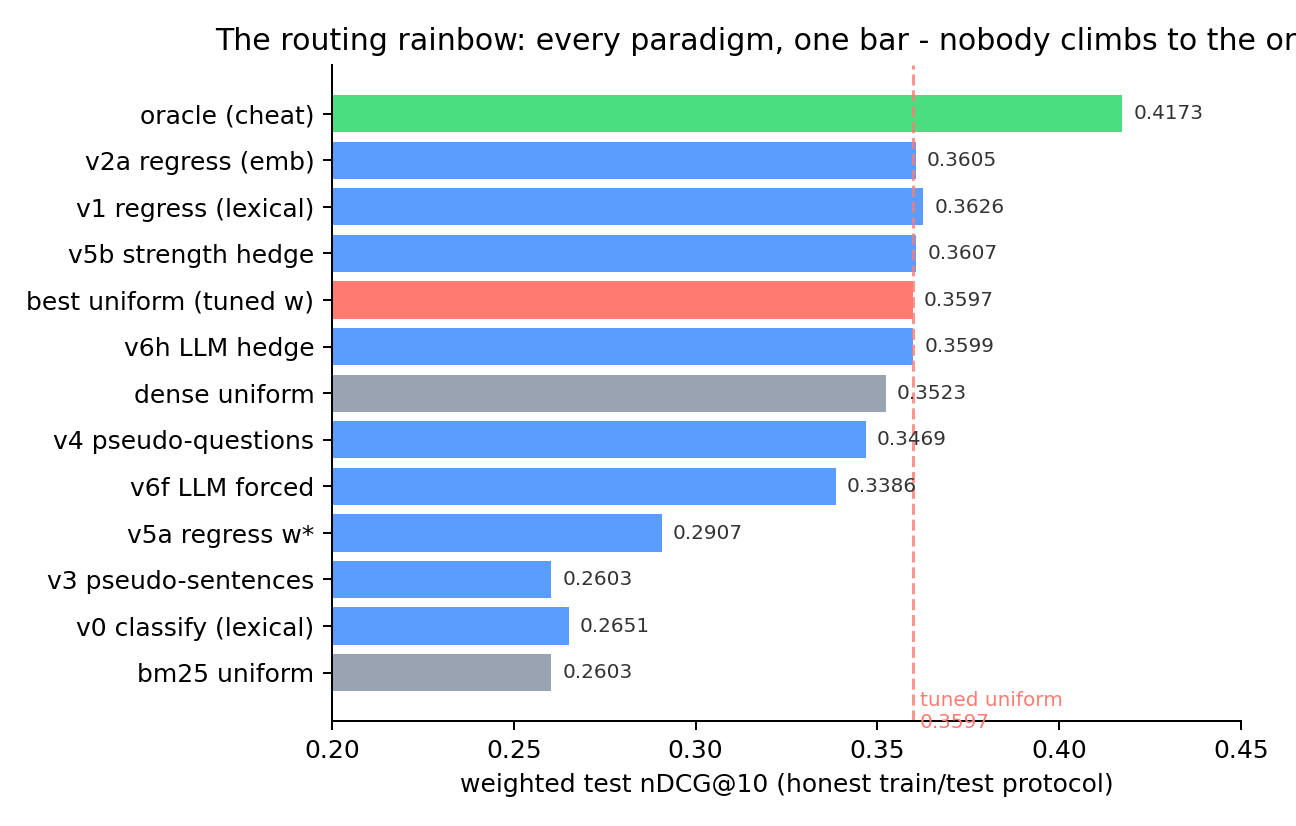
\includegraphics[width=\textwidth]{fig_ladder.png}
\caption{The routing rainbow: every paradigm attempted (blue), fixed baselines (gray), and the oracle (green), on the honest train/test protocol. The dashed line marks the tuned uniform weight --- the bar nobody meaningfully clears.}
\label{fig:ladder}
\end{figure}
\section{Seven attempts to capture the gap}
All routers below are trained on the train split and evaluated once on the test split, per \S2.2. Each subsection reports the outcome \emph{and the mechanism}; the mechanisms are the contribution.

\subsection{Domain routing (the baseline)}
If strategy preference were a property of domains, routing by domain label would capture most of the oracle gap. It captures almost none: routing FiQA$\to$dense, NFCorpus$\to$hybrid yields 0.3580 combined vs 0.3532 for the best single uniform strategy --- \textbf{+1.3\%}. Domain membership explains almost none of the oracle headroom; the signal, if learnable at all, must live in finer-grained properties.

\subsection{v0 --- hard classification on query features}\label{sec:v0}
\textbf{Design.} Six lexical-statistical query features (length, uniqueness, corpus coverage, IDF statistics, stopword count) $\to$ argmax label over strategies, decision tree (depth 4).

\textbf{Outcome.} Collapse: routed 0.2651 vs 0.3532 best uniform (recovery $-181\%$).

\textbf{Mechanism --- tie-breaking bias.} The label was per-query argmax with alphabetical tie-breaking. BEIR train splits carry dense relevance annotations: on such queries all strategies retrieve \emph{something} relevant, per-query scores tie constantly, and alphabetical order resolves every tie to \texttt{bm25}. The pseudo-label means (bm25 0.94, dense 0.55) expose the artifact directly --- and the trained tree routed 96\% of test queries to the worst strategy. \textbf{Lesson:} hard argmax labels on densely annotated training data are a tie-breaking contest, not a learning signal.

\subsection{v1--v2a --- score regression on lexical and embedding features}
\textbf{Design.} Replace hard labels with regression: one model per strategy predicting that strategy's per-query nDCG; route by predicted-score argmax. v1 uses the six lexical features; v2a uses MiniLM query embeddings (PCA-32); v2a-concat uses both.

\textbf{Outcome.} v1: 0.3626 (+0.0028 over uniform; recovery 4.9\%). v2a: 0.3605 (1.4\%). v2a-concat: 0.3624 (4.6\%).

\textbf{Mechanism --- level vs deviation.} The regressors are well-calibrated at the mean --- predicted strategy means track actuals within 0.01 --- but routing needs per-query \emph{deviations}, and the features encode only the \emph{level} (dense $\approx$ hybrid $>$ bm25 everywhere). Two independent feature families converge on the same $\sim$5\% ceiling because the routing signal is not in either representation.

\textbf{Transfer study.} The signal is local. In-sample (train~=~test) recovery is 53.6\% (lexical) and 72.5\% (embedding) --- the information demonstrably \emph{exists} in query features --- but cross-split recovery collapses to $\sim$5\%, and cross-domain transfer at matched distribution is \emph{negative} ($-11.5\%$ and $-25.0\%$ in the two directions, with cross-domain score miscalibration as the visible mechanism). BEIR train splits are not test-distributed; any router trained on them inherits the shift.

\subsection{v3--v4 --- pseudo-labeled training data}
If train splits don't transfer, build training labels from the corpus itself. We generate pseudo-queries with pseudo-qrels (source document = relevant), score all strategies on them with the standard runner, and train the v1 regressors on this per-corpus, test-distributed data.

\textbf{v3} (document sentences as pseudo-queries): routed 0.2603 --- recovery $-181\%$. \emph{Mechanism:} a sentence copied from a document is a perfect lexical match for that document; BM25 wins the pseudo-task \textbf{by construction} (pseudo-label means bm25 0.94--0.96 vs dense 0.55--0.64), and the router learns the pseudo-task, not the real one.

\textbf{v4} (LLM-generated questions as pseudo-queries; Qwen2.5-3B, greedy): routed 0.3469 --- recovery $-22\%$, a four-fold improvement over v3. The generated questions are genuinely question-distributed (the label means compress toward each other; hybrid becomes competitive), confirming the v3 diagnosis --- but the per-query \emph{deviation} signal still does not transfer from pseudo-questions to real ones.

\subsection{v5 --- soft routing: per-query fusion weights}\label{sec:v5}
RCT-MARS (\S\ref{sec:related}) resolves the hard-routing paradox by going soft: predict per-query fusion weights instead of discrete choices. We test both natural variants on our stack.

\textbf{Oracle-soft} (per-query weight grid-searched on test rankings) reaches 0.4237 --- again \emph{above} the hard oracle (0.4173).

\textbf{v5-direct} (regress the optimal weight $w^*$ on query features): 0.2907 weighted ($-24.9\%$ vs uniform). \emph{Mechanism --- the non-convex weight valley.} Per-query nDCG as a function of fusion weight is non-convex (FiQA: $w{=}0.4 \to 0.2714$, $w{=}0.5 \to 0.3574$). The optimal-weight distribution is bimodal --- queries want mostly-BM25 or mostly-dense --- so a conditional-mean regressor predicts middling weights (mean 0.32) that land precisely in the valley where fusion is worst. Soft routing via direct weight regression is a regression-to-the-mean trap on a non-monotonic objective.

\textbf{v5-heuristic} (weight from predicted strategy strengths, $w = \hat{s}_d / (\hat{s}_d + \hat{s}_b)$): 0.3607 (+0.0005). It never hurts and never helps; it behaves like RRF because it \emph{is} RRF in spirit. Once the uniform weight is tuned, hedging has nothing left to add.

\begin{figure}[h]
\centering
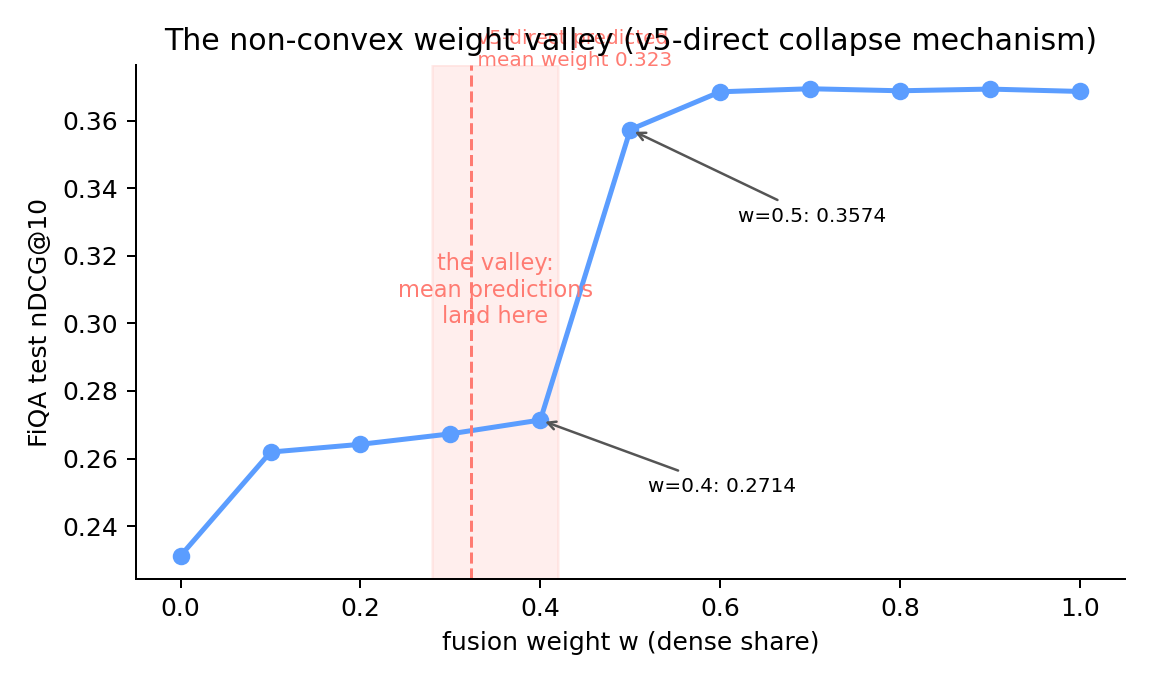
\includegraphics[width=\textwidth]{fig_valley.png}
\caption{Per-query fusion-weight sweep recomputed from committed run artifacts (test split; solid = mean nDCG@10, band = interquartile range across queries). FiQA's mean surface is non-convex --- collapse through $w{=}0.3$--$0.4$, jump at $w{=}0.5$ --- and v5-direct's predicted mean weight (0.323, dashed) lands in the shaded valley: the mechanism of its $-25\%$ recovery. NFCorpus's surface is flatter, consistent with its smaller routing losses.}
\label{fig:valley}
\end{figure}
\subsection{v6 --- LLM-as-router (zero-shot)}
The modern routing literature increasingly uses LLMs as routers. We test zero-shot routing with \texttt{gpt-oss-20b} (Groq), asked to name the best strategy per query from the query text alone, batched and cached; routing uses the committed run artifacts.

Two regimes, both diagnostic:
\begin{enumerate}
\item \textbf{With a hedge option (``hybrid'') in the menu:} the model selects hybrid for 97--100\% of queries --- routing degenerates to the uniform optimum it was meant to beat (+0.0002). Faced with uncertainty, the LLM independently rediscovers our weight sweep's conclusion: \emph{fusion is the safe answer.}
\item \textbf{Forced binary choice} (bm25 vs dense, ``commit to one''): real routing emerges (FiQA: 25\% bm25, 42\% dense, 33\% hybrid-by-parse-fallback) and is decisively \textbf{worse}: $-0.0211$ weighted ($-5.9\%$ relative), $-0.0301$ on FiQA where the model over-routes to BM25. The LLM's priors (``technical terms $\to$ lexical'') are anti-predictive on BEIR --- the same trap as the feature routers, with more confident prose.
\end{enumerate}

Production notes on the LLM router's pipeline fragility (token-budget exhaustion in reasoning models, markdown defeating line parsers, bot-blocking of default HTTP signatures) are relegated to Appendix~B; the scientific finding is the hedging behavior itself.

\subsection{The matrix}\label{sec:matrix}
\begin{table}[h]
\centering\footnotesize
\begin{tabular}{llcccc}
\toprule
\# & router & score & vs uniform & recovery & mechanism \\
\midrule
--- & best uniform (tuned $w$) & 0.3597 & --- & --- & the bar \\
v0 & hard classify (lexical) & 0.2651 & $-26.3\%$ & $-181\%$ & alphabetical tie-bias \\
v1 & score regress (lexical) & 0.3626 & $+0.8\%$ & $+4.9\%$ & level $\neq$ deviation \\
v2a & score regress (embedding) & 0.3605 & $+0.2\%$ & $+1.4\%$ & same ceiling \\
--- & cross-domain transfer & negative & --- & $-11\sim-25\%$ & signal is local \\
v3 & pseudo-sentence labels & 0.2603 & $-27.7\%$ & $-181\%$ & lexical-copy bias \\
v4 & pseudo-question labels & 0.3469 & $-3.6\%$ & $-22\%$ & deviations don't transfer \\
v5a & soft: regress $w^*$ & 0.2907 & $-19.2\%$ & $-25\%$ & non-convex weight valley \\
v5b & soft: strength hedge & 0.3607 & $+0.3\%$ & $+0.1\%$ & $\equiv$ RRF \\
v6h & LLM (hedge allowed) & 0.3599 & $+0.1\%$ & $+0.0\%$ & hedge degeneracy \\
v6f & LLM (forced choice) & 0.3386 & $-5.9\%$ & $-21\%$ & priors anti-predictive \\
\bottomrule
\end{tabular}
\caption{All attempts, honest train/test protocol (test split only), weighted nDCG@10 (baseline uniform 0.3597, oracle 0.4173; all-splits baselines in Table~\ref{tab:baselines}). Baselines recomputed on the canonical test-query set shared across experiments (\texttt{reviewer-stats.md}); per-experiment scores retain their original subsets, hence sub-0.001 wobble.}
\label{tab:matrix}
\end{table}


\section{Why everything ties: a break-even analysis}
The matrix raises the question the failure descriptions cannot answer: is the oracle's headroom a thin sliver that noise drowns, or a real opportunity that predictors keep missing? We characterize every test query: per-strategy scores, oracle = max, best-uniform = the bar; a ``win query'' is one where oracle exceeds the bar.

\textbf{The opportunity is abundant.} The oracle wins on \textbf{54.9\% (FiQA) and 49.5\% (NFCorpus)} of test queries, with mean gains of +0.34 and +0.33 nDCG --- half the benchmark is winnable, and the wins are large.

\textbf{But the break-even accuracy is $\sim$50\%.} With gains that large, the rest of the queries must punish wrong routing comparably --- they do (mean loss $-0.34/-0.27$). The accuracy a router needs to \emph{tie} the uniform baseline is:
\begin{equation}
p^* = \frac{\text{loss}}{\text{gain} + \text{loss}} \;\to\; 49.6\% \text{ (FiQA)},\quad 45.5\% \text{ (NFCorpus)}
\end{equation}

\begin{figure}[h]
\centering
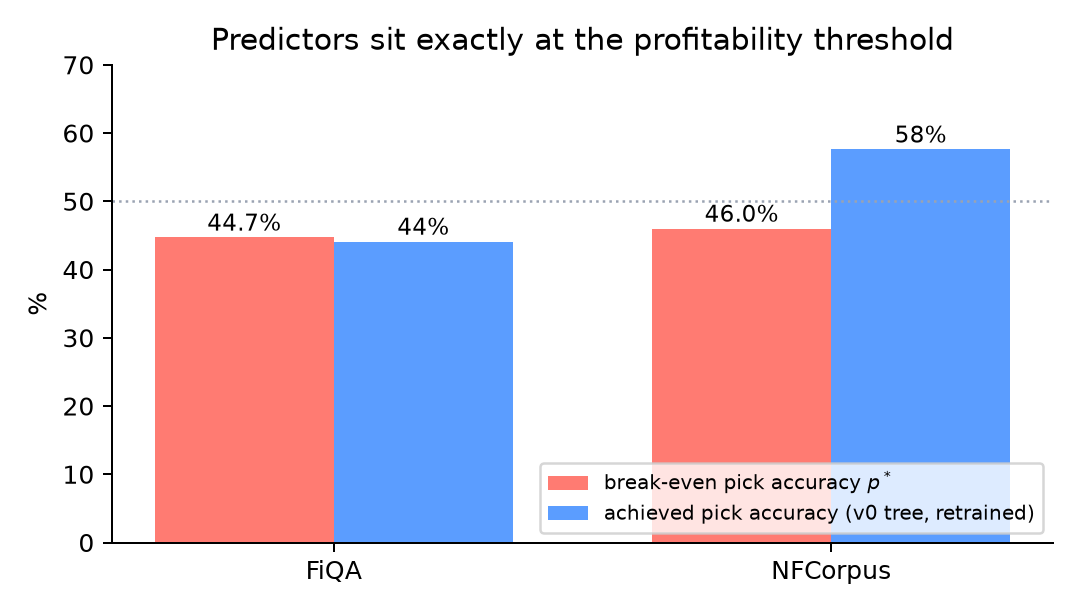
\includegraphics[width=0.75\textwidth]{fig_breakeven.png}
\caption{Break-even pick accuracy $p^*$ (red, from the win analysis) versus the ${\sim}51\%$ accuracy achieved by the best query-feature predictors (blue). Predictors sit at the profitability threshold: expected routing gain ${\approx}$ zero.}
\label{fig:breakeven}
\end{figure}
\textbf{Measured against break-even.} We retrain the paper's best classifier (the v0 decision tree, identical settings) on the canonical query set and bootstrap both quantities over 10{,}000 paired query resamples. Pick accuracy: 48.6\% pooled (95\% CI [45.5, 51.8]); break-even $p^*$: 45.1\% pooled (95\% CI [41.7, 48.5]); $P(\text{acc} > p^*) = 0.95$. Per domain the picture splits: FiQA sits at break-even (44.1\% vs 44.7\%, $P{=}0.41$), while NFCorpus is significantly above it (57.6\% vs 46.0\%, $P{=}0.999$). Routers therefore operate \emph{at or marginally above} the profitability threshold --- and the entirety of what marginally-above buys is the ${\approx}{+}0.003$ pooled gain of Section~4, within noise of the baseline. Query features carry no usable fingerprint: win queries differ only marginally (slightly rarer terms; NFCorpus wins have higher corpus coverage, 0.98 vs 0.81), and the winner mix is split across all three strategies (FiQA wins: dense 193, bm25 100, hybrid 63).

This is the paper's explanatory core: \textbf{predictors operate exactly at the profitability threshold.} The flat results of Section~4 are not a sequence of implementation misfortunes; they are what must happen when a signal exists in-sample (54--72\% recovery proves it does) but its identifying features do not transfer to the deployment distribution. The oracle gap measures how much \emph{knowing the answer} would help --- not how much \emph{reading the question} can.

\textbf{Practical consequence.} A tuned uniform weight requires only a small held-out grid search (we swept 11 values), is robust in the only sense that matters (it cannot be wrong about per-query signals that do not exist), and --- per the oracle-soft result --- the hedging it implicitly performs is what the oracle itself mostly does.

\section{The stakes: strategy choice matters at the answer level}
If no router works, why keep asking the question? Because the \emph{fixed} choice still matters where users feel it. We close the loop at the generation stage: BM25/dense/hybrid (top-5 retrieval) $\to$ Qwen2.5-3B-Instruct answers on 100 FiQA queries, evaluated two ways.

\textbf{Automatic grounding} (relevance-weighted cosine between answer and retrieved sources): 0.501 / 0.631 / 0.574 for bm25 / dense / hybrid.

\textbf{Blind human evaluation.} 90 judgments (30 queries $\times$ 3 strategies, shuffled, strategy hidden), graded Correct / Partial / Wrong against the retrieved sources by one rater (Table~\ref{tab:human}).

\begin{table}[h]
\centering\small
\begin{tabular}{lcccc}
\toprule
strategy & Correct & Partial & Wrong & correct-rate (95\% CI) \\
\midrule
bm25   & 26 & 4 & 0 & 86.7\% [69.3, 96.2] \\
dense  & 29 & 1 & 0 & 96.7\% [82.8, 99.9] \\
hybrid & 28 & 2 & 0 & 93.3\% [77.9, 99.2] \\
\bottomrule
\end{tabular}
\caption{Blind human evaluation, 30 FiQA queries $\times$ 3 strategies.}
\label{tab:human}
\end{table}

The human ordering (dense $>$ hybrid $>$ bm25) exactly preserves the grounding-proxy ordering --- two independent measurement levels, one conclusion. Failures concentrate in Partial (missed key points), and 4 of the 5 Partials belong to BM25 --- thin retrieval propagating into incomplete answers, the human-visible form of the routing mechanism. Caveats honestly noted: $n{=}30$ per strategy with overlapping CIs (directional, not powered for superiority); the sample derives from the first 100 queries and is topically clustered.

\section{Related work}\label{sec:related}
\textbf{The routing paradox.} RCT-MARS (Springer JIIS, 2026; independent, concurrent) establishes on six benchmarks and five retrieval paradigms that learned hard routers fall below the strongest fixed method despite a large oracle ceiling, and that \emph{soft} routing (learned fusion weights, CASR) recovers +16.4\% of the gap, matching RRF. Our study replicates the paradox independently on BEIR with a three-strategy stack, extends it to soft routing (which fails on our train/test protocol --- most directly via the weight-valley mechanism), adds the seven-attempt mechanism matrix, the break-even theory, and the human evaluation. Where RCT-MARS asks ``what makes routing succeed?'', we ask ``why does every paradigm fail, exactly?'' --- the two papers are complementary, and our stack-level disagreement (their soft routing works; ours does not transfer) is itself informative: the viability of soft routing appears to depend on training data that matches the deployment distribution, which BEIR train splits are not.

\emph{A note on the apparent disagreement.} RCT-MARS's learned soft router \emph{matches RRF} --- and RRF is itself a constant fusion rule. Our best fixed strategy \emph{is} a tuned fusion weight, against which matching-RRF has nothing to gain. The delta between the two studies is therefore less ``soft routing succeeds vs.\ fails'' than ``what counts as the fixed baseline'': where the strongest fixed method is already fusion, soft routing's known ceiling (RRF-equivalence) coincides with the baseline. A faithful CASR replication under the BEIR split protocol remains future work; our claims are scoped to the stacks and protocols we tested.

\textbf{LLM routing.} RouteLLM (Ong et al., 2024) routes between strong and weak LLMs with a trained classifier, successfully --- but its supervision is drawn from the \emph{same deployment distribution} it serves, the one condition our transfer study shows is necessary. RAGRouter (2025) routes among RAG pipelines with oracle upper bounds reported; our v6 supplies the missing controlled counterpoint: zero-shot LLM routing on BEIR is either degenerate (hedge) or harmful (forced choice).

\textbf{Adaptive retrieval.} Mallen et al.\ (2023) decide \emph{whether} to retrieve per query using a classifier trained on same-distribution Wikipedia supervision --- again the workable regime. Our per-query \emph{strategy} routing differs in the action space but shares the lesson: the training distribution is the whole game.

\textbf{Synthetic query generation.} InPars (Bonifacio et al., 2022) generates LLM queries from documents to \emph{train retrievers} --- and works, because representation learning generalizes where per-query comparative labels (our routing targets) do not. Our v3$\to$v4 contrast is the cautionary complement: the same generation pipeline, used to label \emph{routing decisions}, exposes how fragile the pseudo-task is (a $-181\%$ collapse from lexical-copy bias that a naive reading would call ``BM25 is best'').

\textbf{Fusion.} Reciprocal Rank Fusion (Cormack et al., 2009) and its modern descendants establish that simple rank combination is a stubbornly strong baseline; our weight sweep and v5b reproduce this in the routing frame. BEIR (Thakur et al., 2021) documents the cross-domain fragility of dense retrieval that our transfer study quantifies specifically for routing decisions.

\section{Limitations}
\begin{enumerate}
\item \textbf{Scale.} Two datasets and three strategies; RCT-MARS' broader stack may admit routers ours cannot. Our conclusions are conditioned on BEIR-style train/test separation --- which is also the setting most routing evaluations actually use.
\item \textbf{Human evaluation.} One rater, $n{=}30$ per strategy, overlapping CIs; directional rather than definitive.
\item \textbf{Feature scope.} Six lexical features and one embedding model; richer features might squeeze past break-even, though the in-sample-vs-transfer gap suggests the bottleneck is distribution shift, not representation.
\item \textbf{Label quality.} Pseudo-labels and LLM routers each carry their own noise; we mitigated but cannot eliminate it.
\item \textbf{All-splits baselines} are used for published-number comparability; router conclusions rest on the honest split protocol, and the two are clearly delineated.
\end{enumerate}

\section{Conclusion}
We set out to harvest the oracle gap and ended up measuring why it cannot be harvested. The oracle's promise is real --- abundant wins, large margins, a soft ceiling even higher than the hard one. But the wins carry no query-side fingerprint beyond chance, and so every router paradigm, from six-feature regression to zero-shot LLM judgment, operates at or negligibly above the profitability threshold the break-even analysis predicts (pooled $P(\text{acc} > p^*) = 0.95$). The mechanisms we documented along the way --- tie-bias collapse, level-vs-deviation, lexical-copy pseudo-labels, the weight valley, hedge degeneracy --- are individually useful warnings and collectively a map of where not to look.

The uncomfortable recommendation survives every robustness check we could throw at it: \textbf{sweep the fusion weight once, then stop routing.} And the oracle gap, henceforth, should be read for what it is --- an upper bound on hindsight, not a forecast for routing.

\appendix
\section{Artifact guide}
Repository: \url{https://github.com/ChefSanto/rags}. Everything in this paper reproduces from a fresh clone:
\begin{itemize}
\item \texttt{experiments/configs/} --- every experiment as YAML (baselines, sweep, Qwen generation, pseudo-labels).
\item \texttt{experiments/results/} --- committed result JSONs (with provenance) and analysis reports: \texttt{oracle-*.md}, \texttt{domain-router-*.md}, \texttt{router-v0}\dots\texttt{router-v6-*.md}, \texttt{routing-wins-*.md}, \texttt{human-eval-fiqiqa-30q.csv}.
\item \texttt{artifacts/runs/} --- ranked run artifacts for all baselines (oracle, domain-router, v5, v6, and win analyses read these directly).
\item \texttt{scripts/} --- runner, oracle/domain analyses, routers v0--v6, pseudo-query generators, win analysis, review-sheet generator.
\item \texttt{core/} --- retrieval, evaluation (incl.\ per-query metrics), generation, schema.
\item The same repository deploys a working RAG (Cloudflare Workers + Vectorize + D1) with a chat dashboard over the FiQA corpus and user-uploaded documents --- the platform whose benchmarking produced this paper.
\end{itemize}
Reproduce the headline results: \texttt{bash scripts/kaggle\_bootstrap.sh} (Kaggle; idempotent), then \texttt{python scripts/oracle\_analysis.py --dataset fiqa --metric ndcg\_at\_10}, \texttt{python scripts/router\_v5\_soft.py --datasets fiqa nfcorpus}, \texttt{python scripts/routing\_win\_analysis.py --datasets fiqa nfcorpus}.

\section{LLM-router pipeline fragility}\label{app:fragility}
Getting the LLM router to answer at all required diagnosing three production failures, each invisible in feature-based routers: (1)~reasoning models (\texttt{gpt-oss-20b}) exhausted the completion token budget on deliberation, returning empty responses until \texttt{reasoning\_effort: low} was set; (2)~markdown-formatted answers (\texttt{**1.** bm25}) defeated line-anchored parsers, silently degrading to the fallback label until the parser was made markdown-tolerant; (3)~Cloudflare's bot-management rejected the default \texttt{Python-urllib} client signature with HTTP 403 (error 1010), requiring an explicit client User-Agent. These are integration costs of LLM routers, noted for reproducibility.

\section*{Acknowledgments}
The author thanks the Kaggle free GPU tier and Cloudflare's free/paid Workers tiers, under which the entire platform and evaluation ran at trivial cost; and the anonymous engineers of every API version bump encountered along the way, each of which taught a lesson this paper needed.

\end{document}
